\documentclass[tikz]{standalone}
\usepackage{amsmath,amssymb}

\newcommand{\twovec}[2]{\ensuremath{\begin{pmatrix}{#1}\\{#2}\end{pmatrix}}}
\newcommand{\V}[1]{\vec{\mathbf{#1}}}

\tikzset{mydraw/.style={black,->}}
\tikzset{mynode/.style={scale=0.7}}

\begin{document}
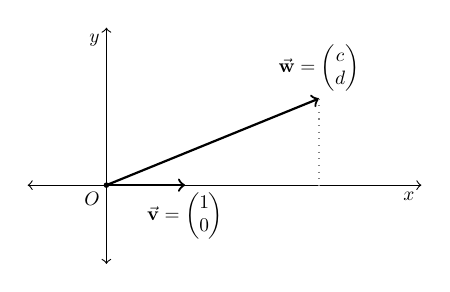
\begin{tikzpicture}
	\clip (-1,-1) rectangle (4,2);

	\draw[mydraw] (0,0) -- (-1,0);
	\draw[mydraw] (0,0) -- (0,-1);
	\draw[mydraw] (0,0) -- (4,0) node[mynode,below left] {\(x\)};
	\draw[mydraw] (0,0) -- (0,2) node[mynode,below left] {\(y\)}; % axis lines

	\draw[thick,->] (0,0) -- (1,0) node[mynode,below] {\(\V{v} = \twovec{1}{0}\)};
	\draw[thick,->] (0,0) -- (2.7,1.1) node[mynode,above] {\(\V{w} = \twovec{c}{d}\)};

	\draw[gray, dotted] (2.7,1.1) -- (2.7,0);

	\fill[black] (0,0) circle (1pt) node[mynode,below left] {\(O\)};
\end{tikzpicture}
\end{document}
